\chapter{ Решеточные модели в статистической физике }
\label{ch:ch1}
 
В данной главе формализованы спиновые модели на динамической геометрии, генерируемой блужданиями без самопересечений (БСП) фиксированной длины на регулярной решетке. 
Рассматриваются гамильтонианы моделей Изинга и XY и набор наблюдаемых. 
Эти определения будут использоваться в последующих главах.


\paragraph*{Модели в статистической физике.}

 Модели задаются гамильтонианом --- функцией энергии, определяющей вероятностное распределение состояний. 
 Гамильтониан спиновых  моделей на динамических структурах зависит одновременно от конфигурации спинов $s$ и их пространственного расположения  (конфигурации БСП $u$). 
 В отсутствии действия внешнего поля задается следующим образом:
 
 \begin{equation}
 	\label{hamiltonian}
 	  H(s, u) = -J \sum_{ \langle i, j \rangle \in \mathcal E } e_{ij},  %- h \sum_i s_i,
 \end{equation}
    где постоянный параметр  $J>0$ моделирует обменное взаимодействие между спинами, $ e_{ij}$ -   взаимодействия спиновых переменных $i $  и $j$ (вклад пары спинов).  
    Здесь $\mathcal E$ — множество взаимодействующих неповторяющихся пар.  
    Для  случая ближнего взаимодействия $\mathcal E$ — пары ближайших соседей. 
    Для случая дальнего взаимодействия  вместо выбора $\mathcal E$ используют весовую сумму:  $ H(s, u) =-\,J\sum_{i<j} K(r_{ij})\,e_{ij},$
    где $K(r)$ — убывающее ядро (например, степенное), $r_{ij}$ — выбранная метрика.
    
  
В данной работе при изучении спиновых моделей на динамической геометрии (Изинга и XY) рассматривается  \textit{канонический ансамбль} при фиксированной длине $N$: геометрия пробегает множество $\mathcal U_N$ всех допустимых конфигураций длины $N$, спины — своё пространство $\mathcal S$. Статистическая сумма тогда имеет вид:

 \begin{equation}
 	\label{Zcanonical}
 	Z_N = \sum_{u\in \mathcal U_N} \ \sum_{s\in \mathcal S} \exp\!\big[-\beta H(s,u)\big], 
 	\qquad \beta=\frac{1}{k_B T},
 \end{equation}
где $k_B$ — постоянная Больцмана. 
Знак $\sum_{s}$ трактуется широко: для непрерывных спинов он означает интегрирование по естественной нормированной мере. 
Без потери общности примем \(\beta=1\) (энергии тогда измеряются в единицах \(k_B T\)).
   
   Соответствующее распределение Больцмана-Гиббса имеет вид:
   \begin{equation}
   	\label{gibbs}
   	P_N(s,u)=\frac{1}{Z_N}\,\exp\!\big[ -H(s,u)\big],
   \end{equation}
   а математическое ожидание наблюдаемой величины $	\langle \mathcal O\rangle_N$ выражается через множества $\mathcal U_N$ и   $\mathcal S$ следующим образом:
   \begin{equation}
   	\langle \mathcal O\rangle_N=\sum_{u\in \mathcal U_N}\ \sum_{s\in \mathcal S} \mathcal O(s,u)\,P_N(s,u).
   \end{equation}
   
   
 \section{ Блуждание без самопересечений (БСП)}\label{sec:2_ch:1}
 
Решеточные модели полимеров --- стандартный инструмент изучения критических явлений и моделирования полимеров  \cite{Rensburg} \cite{Vanderzande_1998}. 

Линейный полимер --- это длинная макромолекула, состоящая из мономеров. 
Основным подходом для моделирования геометрии (конформации) линейных полимеров в статистической физике являются блуждания без самопересечений (БСП, Self-Avoiding Walk, или SAW, в англоязычной научной литературе). 
Пример такой конформации показан на рисунке \ref{fig:homopolymer}. 
Модель блуждания без самопересечений хорошо описывает полимерную цепочку благодаря учёту «эффекта исключённого объёма»:  отсутствие  пересечений шагов блуждания на решетке  моделирует отталкивание мономеров, связанное с силами Ван-дер-Ваальса   \cite{Schfer2011ExcludedVE} \cite{Binder_Sokal_chapter}.

Геометрия полимерной цепочки длины $N$ ---  это блуждание без самопересечений (БСП), состоящее из  $N$ вершин (узлов) на регулярной решетке, соединенных последовательно с помощью $N-1$ ребра.
 
\begin{figure}
    \centering
 	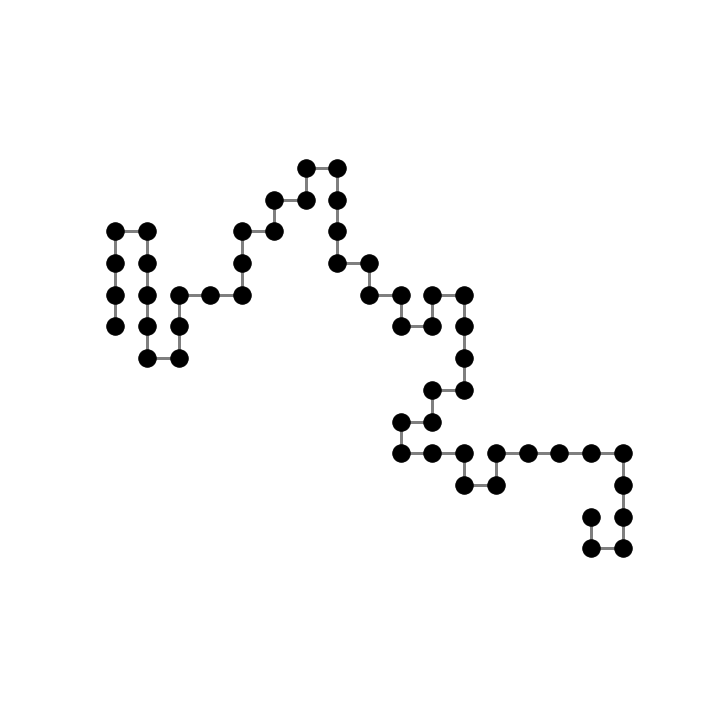
\includegraphics[width=0.35\textwidth]{images/homopolymer}
 	\caption{Пример конформации (геометрии) гомополимера, состоящего из одинаковых мономеров.}
 	\label{fig:homopolymer}
\end{figure}  

 Модель гомополимера (БСП) испытывает фазовый переход от "клубка" (coil, развернутого состояния) к "глобуле" (globule, свернутому состоянию), являющийся важным феноменом в статистической теории полимеров. 
 В теории полимеров, глобулярная форма соответствует состоянию цепочки в плохом растворителе, а развернутая форма --- полимеру в хорошем растворителе \cite{Scaling_concepts}. 


Главный интерес к модели гомополимера связан с её критическим поведением, определяющим масштаб полимера (размер полимера) и универсальные показатели.  
Критические индексы отражают универсальное поведение, независимое от микроскопических деталей.   

Для описания  структурного состояния полимера используют геометрические параметры.
Одними из таких параметров являются среднее расстояние между концами БСП (средний радиус, end-to-end distance) и радиус инерции (вращения, gyration radius).

Рассмотрим конформацию $u$ c координатами вершин ${r_1, r_2, \dots, r_N}$. 
Тогда средний радиус определяется следующим образом: 

\begin{align}
	\label{endtoend}
	R &=  |\mathbf R| = | r_N - r_1 |  	\quad  R^2=\lvert \mathbf R\rvert^2     \\
	\langle R_N^2 \rangle  &=  \frac{1}{Z_N^{\text{SAW}}} \sum_{  u \in  \mathcal U_N }  |\mathbf R|^2 e^{-H(u)},
\end{align}

где $|\mathbf R|$ - евклидово расстояние между концами конформации  $u$,  $Z_N^{\text{SAW}} =  \sum_{u\in \mathcal U_N}  \;\exp\!\big[-\,H(u)\big] $ - статистическая сумма  канонического ансамбля по всем конфигурациям длины $N$. 

Радиус инерции  определяется как среднее квадрата расстояний всех мономеров до центра масс цепочки $r_{cm}=\frac{1}{N}\sum_{i=1}^N r_i$:

\begin{align}
	\label{gyration}
	%R_g = \frac{1}{N} \sum_{i=1}^N  |r_i - r_{cm}|  	\quad  
	R_g ^2 = \frac{1}{N} \sum_{i=1}^N  |r_i - r_{cm}|  ^2     \\
		\langle R_{g, N}^2 \rangle  =  \frac{1}{Z_N^{\text{SAW}}} \sum_{  u \in  \mathcal U_N }  R_g ^2 e^{-H(u)},
\end{align}

В термодинамическом пределе  $N \rightarrow \infty $,  оба средних радиуса подчиняются степенному закону: 
\begin{align}
	\label{r_scale}
	\langle R_N^2 \rangle \sim N^{2 \nu } ,	\quad 
		\langle R_{g, N}^2 \rangle \sim N^{2 \nu }. 
\end{align} 

Здесь ${\nu} $  - критический показатель. Далее рассмотрим  значения критических  экспонент  в двумерном и трёхмерном случаях.  

 


\subsection{Двумерный случай}\label{homopolymer_2d} 

Рассмотрим случай классической модели - гомополимера,  у которого все узлы состоят из одинаковых мономеров, т.е. нет спиновой динамики. 
В случае отсутствия межспинного обмена  $J=0$ в \eqref{hamiltonian} (режим высокой температуры/сильный растворитель), любая спиновая модель на БСП эквивалентна невзаимодействующему гомополимеру.
  Для таких моделей ($J=0$) найдено точное решение для значения критической экспоненты $\nu$   аналитически \cite{PhysRevLett.49.1062} и подтверждено численно с большой точностью \cite{li1995critical}   :    % \cite{van2015statistical}  
\begin{equation}
	\label{nur}
	\nu = \frac{3}{4}. 
\end{equation}

 

В  ${\theta}$-точке (фазовый структурный переход), значение показателя  $\nu$  получено аналитически (методом приближений) \cite{PhysRevLett.57.941} и численно \cite{Caracciolo_2011}: 
\begin{equation}
	\label{nu_theta}
	\nu_{\theta} = \frac{4}{7}.
\end{equation}  
 

В глобулярной фазе: 

\begin{equation}
	\label{globular}
	\nu = \frac{1}{d} = \frac{1}{2},
\end{equation} 
так как при низкой температуре (или слабом растворителе), полимер сжат в глобулу и занимает наименьший объем, то есть круг.

\subsection{Трехмерный случай}\label{homopolymer_3d}  


Для случая $J=0$, изначально критический показатель был оценен приближением Флори:   \cite{flory1953principles}: 
\begin{equation}
	\label{eq:nu_3D_J0_flory}
	\nu = \frac{3}{2+d} = \frac{3}{5}.
\end{equation}
В дальнейшем, оценка показателя  $\nu$  для отсутствия взаимодействия была также сделана  численно \cite{li1995critical}:
\begin{equation}
	\label{eq:nu_3D_J0_sokal}
	\nu = 0.5877 \pm 0.0006.
\end{equation}

 
В  ${\theta}$-точке, показатель $\nu$ также найден аналитически  \cite{Vanderzande_1998} и численно  \cite{barat1993series}: 

\begin{equation}
	\label{eq:nu_3D_Jtheta_flory}
	\nu = \frac{1}{2}.
\end{equation} 


В режиме $J > J_{\theta}$,  макромолекула  коллапсирует в компактную глобулу  и стремится занять наименьший  объем --- сфера в трехмерном пространстве, следовательно, показатель $\nu$  следующий:  
\begin{equation}
	\label{eq:nu_3D_Jglobular_flory}
	\nu = \frac{1}{d} = \frac{1}{3}.
\end{equation}

 
 
  %\subsection{Фазовые переходы в полимерных моделях}
  
  \section{Динамическая гидрофобно-полярная (HP) модель полимера}
  \label{sec:2_ch:hp}
 
 Одна из простейших классических моделей полимерной цепочки (гетерополимера) -- гидрофобно-полярная  (HP) модель  \cite{lau1989lattice}, первоначально разработанная для моделирования процесса сворачивания белков \cite{Khalatur1998, Khalatur2012}. 
 В такой модели, каждый мономер может быть либо гидрофобным ($H$), либо полярным ($P$). В задачах моделирования сворачивания белка последовательность   мономеров, как правило, фиксирована, а геометрия цепи является динамической.
 
 В рамках данного исследования рассматривается  динамическая HP-модель на квадратной решётке. Полимерная цепь задаётся самонепересекающимся блужданием длины $N$.
 Каждый мономер может находиться в одном из двух состояний: гидрофобном ($H$) или полярном ($P$), а состояние мономера динамичное. 
 
 
 
 \begin{figure}[h!]
 	\centering
 	\includegraphics[scale=0.44]{HP_example_cut.png}
 	\caption{ Пример цепочки длины $N=11$, чья конформация содержит $m=2$ топологических H-H контакта. Пример последовательности: HPHHHPPPPHH.}
 	\label{fig:saw_example}
 \end{figure}
  
 
 Если два мономера занимают соседние узлы решётки, но не являются соседями вдоль цепи, то говорят, что они образуют \textit{топологический контакт}. Взаимодействие возникает только между контактами типа $H$-$H$. Каждый такой контакт даёт вклад в энергию $-\epsilon_b<0$. Контакты $P$-$P$ и $P$-$H$ в энергию  вклад не вносят. Пример показан на рисунке \ref{fig:saw_example}. 
 
 Энергия фиксированного состояния  $u$ для большого канонического ансамбля  определяется следующим выражением: 
 \begin{equation}
 	E_u = -\epsilon_b m - \epsilon_a N,
 \end{equation}
 где $m$ --- число топологических контактов $H$-$H$, а $\epsilon_a$ --- химический потенциал, связанный с длиной цепи.
 
 Статистическая сумма в большом каноническом ансамбле имеет вид
 \begin{equation}
 	Z=\sum_{N=0}^{\infty}\sum_u e^{-E_u/kT}
 	= \sum_{N=0}^{\infty}\sum_u x^m \beta^N,
 \end{equation}
 где
 \begin{equation}
 	\beta = e^{\epsilon_a/kT}, \qquad x=e^{\epsilon_b/kT}.
 \end{equation}
 
Без потери общности выбирается единица энергии так, что $kT=1$.
  
  Критическое значение химического потенциала  в данной модели зависит от параметра взаимодействия $x$:
  \begin{equation}
  	\beta_c=\beta_c(x).
  \end{equation}
  Исследование зависимости $\beta_c(x)$ позволяет определить границу между различными режимами системы. 
 
 
\section{ Спиновые модели  на динамических структурах}\label{sec:1_ch:1}
 
Спиновые переменные могут принимать дискретные значения или непрерывный диапазон.  
В качестве дискретного и непрерывного вариантов спиновых переменных мы рассмотрим соответственно модели Изинга и XY на динамических структурах, генерируемые блужданиями без самопересечений (БСП) на регулярных решетках. 
 
 \subsection{  Модель Изинга на динамических структурах}\label{sub1:sec:1_ch:1}
 

 Модель Изинга — одна из простейших и наиболее изученных моделей в статистической физике. 
 
 Мы рассматриваем модель Изинга на динамических структурах, порождаемые  блужданиями без самопересечений  \ref{sec:2_ch:1}. 
 
 \begin{figure}
 	\centering
 	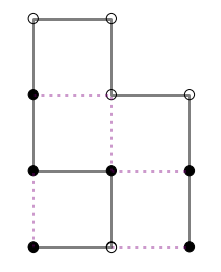
\includegraphics[width=0.35\textwidth]{images/onlysaw}
 	\caption{Пример состояния: 2 вида спинов на блуждании без самопересечений. Сплошной серый цвет ребер - последовательные соединения, пунктирные фиолетовые - топологические.}
 	\label{fig:ising_example}
 \end{figure}  
 
 
  Каждый  спин принимает одно из двух дискретных значений: $s_i = \pm 1$.  Гамильтониан - сумма по всем взаимодействующим парам спинов $\langle i, j \rangle $, включая и  последовательные пары цепи и контактные пары на расстоянии 1 на решётке, как показано на примере  \ref{fig:ising_example}, в соответствии c конформацией  БСП $u$:
  \begin{equation}
  	\label{hamiltonian_ising}
  	  H(s, u) = -J \sum_{ \langle i, j \rangle } s_i s_j     
  \end{equation}
 
  
   Статистическая сумма канонического ансамбля \eqref{Zcanonical} --- проход всевозможных спиновых последовательностей  $s$, состоящих из  $+1$ или $-1$ (всего их $2^N$)  и всех БСП  $u \in\mathcal U_N$  длины $N$:
 
  \begin{equation}
  	Z_N(J)=\sum_{u\in\mathcal U_N}\ \sum_{s\in\{\pm1\}^N}\exp\!\Big[J\sum_{(i,j)\in\mathcal E(u)} s_i s_j\Big] .
  \end{equation}
  
%Средняя намагниченность на спин в модели Изинга определяется как среднее по спиновым состояниям:

 
 Параметр порядка задается как модуль намагниченности на спин:
 \begin{equation}
 	 	\label{ising_mean_magnetization}
 	m(s)=\frac{1}{N}\Big|\sum_{i=1}^N s_i\Big|,\qquad 
 	\langle m\rangle=\frac{1}{Z_N}\sum_{u,s} m(s)\,e^{-H(s,u)}.
 \end{equation}
 
 
 
  \subsection{  Модель XY на динамических структурах}\label{sub2:sec:1_ch:1}
 
 
 Модель XY является классической моделью с непрерывными спиновыми переменными \cite{kosterlitz1973ordering}. 
 
Каждый $i$-ый узел БСП хранит непрерывное значение спина $s_i$, которое задает угол  $\theta_i \in  [-\pi;\pi]$. 
Спины в модели XY --- единичные векторы на окружности: $s_i=(\cos\theta_i,\sin\theta_i)$
Примеры состояний для двумерного случая  показаны на рисунке \ref{fig:example_xy}, для трехмерного случая --- на графике \ref{fig:example_xy_3d}.  
 


  \begin{figure}
 	\centering
 	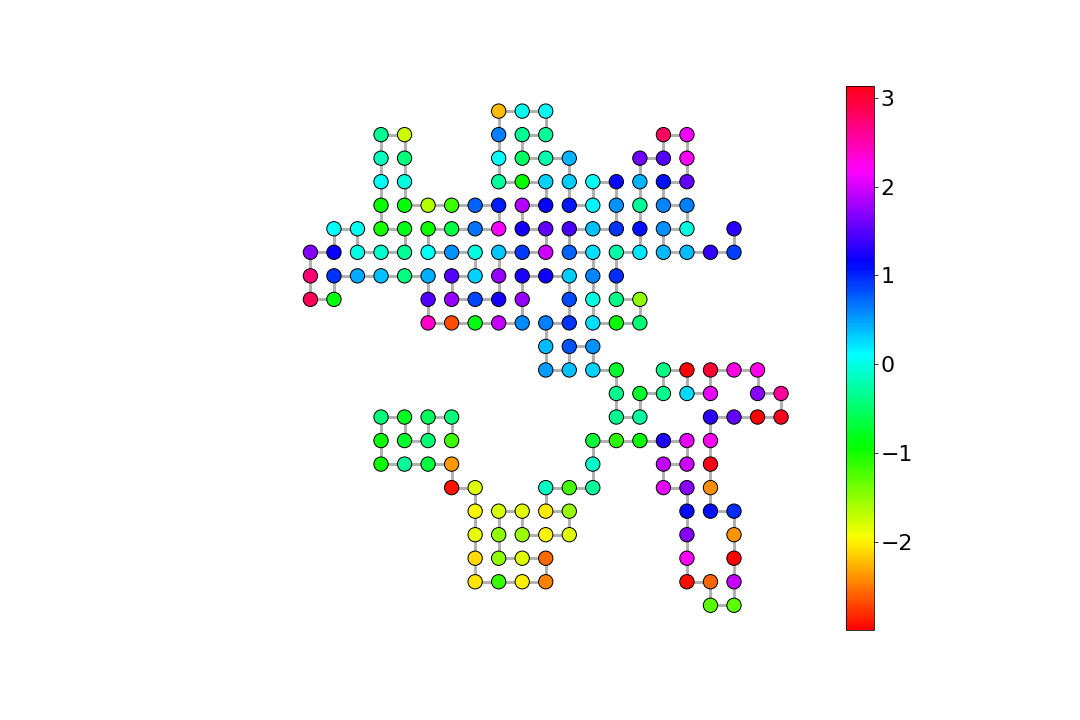
\includegraphics[scale=0.20]{images/state_example.png}
 	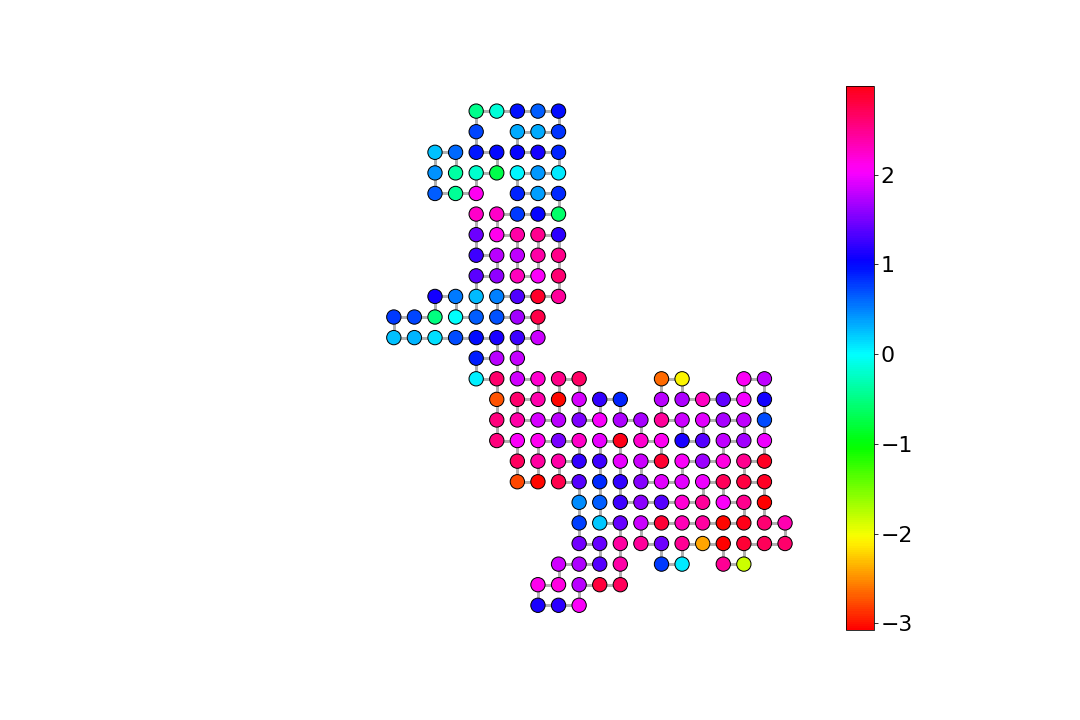
\includegraphics[scale=0.20]{images/state_example1.png} 
 	\caption{ Пример состояний цепочки $N=200$ на квадратной решетке, полученные  численным моделированием.  Цветом показаны значения спинов --- угол  $\theta_i$. }
 	\label{fig:example_xy}
 \end{figure}
 
 
\begin{figure}%\vspace{1cm}
 	\includegraphics[width=0.23\linewidth]{state_coil.png}
 	\includegraphics[width=0.23\linewidth]{state_coil_1.png}
 	\includegraphics[width=0.23\linewidth]{state_glob.png}
 	\includegraphics[width=0.253\linewidth]{state_glob_1.png}
 	\captionof{figure}{Пример состояний цепочки $N=400$ на кубической решетке, полученные  численным моделированием.  Цветом показаны значения спинов --- угол  $\theta_i$.}
 		\label{fig:example_xy_3d}
 \end{figure}%\vspace{1cm}
 
В отсутствии внешнего поля, Гамильтониан для состояния спиновой последовательности  $s$ на конформации  $u$ определяется как сумма взаимодействующих пар  спинов  $\langle i, j \rangle$ на БСП через косинус разности их угловых переменных:
 \begin{equation}
 	\label{hamiltonian_xy}
 	H(u,s) = -J \sum_{ \langle i, j \rangle } \cos(\theta_i - \theta_j).  
 \end{equation} 
  
  
  Статистическая сумма канонического ансамбля \eqref{Zcanonical}  для цепочки длины $N$  --- сумма по всему пространству  конфигураций $u$ заданной длины и всему спиновому пространству:  
  
    \begin{equation}
   	\label{partitionfunction2}
  Z_N(J)
  = \sum_{u\in\mathcal U_N}
  \int_{(-\pi,\pi]^N}
  \left[\prod_{(i,j)\in\mathcal E(u)} e^{\,J\cos(\theta_i-\theta_j)}\right]
  \prod_{i=1}^N \frac{d\theta_i}{2\pi}.
  \end{equation}

%  \begin{equation}
% 	\label{partitionfunction2}
% 	Z(J) =  \sum_{u \in \mathcal U_N }  \int_{-\pi}^{\pi}   \frac{   d \theta_1  d \theta_2 \dots   d\theta_N }{ (2 \pi  )^N}
% 	\prod_{ \langle i, j \rangle  }^{  }   \left[  e ^{    J    \cos(\theta_i - \theta_j)    }     \right] ,            
%  \end{equation} 
% 
% Средняя намагниченность на спин в модели XY определяется как среднее по спиновым состояниям:
% \begin{equation}
% 	\label{xy_mean_magnetization}
% 	\langle m \rangle =   \frac{1}{N}  \sqrt{       \langle  ( \sum_i^N \cos \theta_i  )^2      + ( \sum_i^N    \sin \theta_i   )^2             \rangle    }. 
% \end{equation}
 
  
 Вектор намагниченности и параметр порядка:
 \begin{equation}
 		\label{xy_mean_magnetization}
 	\mathbf M(s)=\frac{1}{N}\sum_{i=1}^N (\cos\theta_i,\sin\theta_i),\qquad m(s)=|\mathbf M(s)|,\qquad \langle m\rangle=\frac{1}{Z_N}\sum_{u}\int m(s)\,e^{-H}\,d\mu.
 \end{equation}
  \begin{equation}
 \langle m^2\rangle
 = \Big\langle M_x^2+M_y^2\Big\rangle
 = \frac{1}{N^2}\Big\langle \Big(\sum_{i=1}^N \cos\theta_i\Big)^2
 + \Big(\sum_{i=1}^N \sin\theta_i\Big)^2 \Big\rangle
  \end{equation}
  
 \subsection{Фазовые переходы в спиновых системах} 
 
 % Определения экспонент
 % ν_SAW: геометрический (R ~ N^{ν_SAW})
 % ν_spin: спиновый (ξ ~ |J-J_c|^{-ν_spin})
 \newcommand{\nuSAW}{\nu_{\mathrm{SAW}}}
 \newcommand{\nuSpin}{\nu_{\mathrm{spin}}}
 \newcommand{\nuEff}{\nu_{\mathrm{eff}}}
 
Для определения типа фазового перехода используются кумулянты Биндера четвертого порядка для намагниченности \eqref{xy_mean_magnetization},  \eqref{ising_mean_magnetization} \cite{PhysRevLett.47.693}: 


  \begin{equation}
 	\label{binder_cumulant}
  U_4 = 1 - \frac{ 	\langle m^4 \rangle  }{ 3 	\langle m^2 \rangle ^2 }. 
 \end{equation}
 
 Критерий перехода второго рода: кривые $U_4^N(J)$ для систем разного размера $N$ пересекаются в одной точке $J_{critical}$.   
 
 Спиновая корреляционная длина в окрестности $J_{critical}$ ведёт себя как
 \[
 \xi(J)\;\sim\; |J-J_{critical}|^{-\nu_{\mathrm{spin}}}.
 \]
 
 На динамической геометрии естественный линейный размер системы — это $N_{\mathrm{eff}}(N)\sim R(N)\sim N^{\nu_{\mathrm{SAW}}}$. 
  Удобно ввести эффективный показатель по N:
 \[
 \frac{1}{\nuEff} \equiv \frac{\nuSAW}{\nuSpin}
 \quad\Longleftrightarrow\quad
 \nuEff = \frac{\nuSpin}{\nuSAW}.
 \]
  
 В критической области выполняется  масштабирование 
\[
U_4(J,N)
= \mathcal U\!\Big( (J-J_{critical})\, N^{1/\nuEff} \Big)
+ \mathcal O\!\big( N^{-\omega_{\mathrm{eff}}} \big),
\qquad
\left.\frac{dU_4}{dJ}\right|_{J=J_{critical}} \sim N^{1/\nuEff}.
\]
  а само критическое значение $U_4^\star$ зависит от граничных условий и формы системы (т.е. не «универсально» в строгом смысле) \cite{selke2006critical}.
   Для переходов типа БКТ (модель XY на регулярной квадратной решетке) поведение $U_4$ осложнено логарифмическими поправками \cite{hasenbusch2008binder}. 
  
 
 Критерий для фазового перехода первого рода: кривые кумулянта имеют отрицательный минимум $U_4^{\min}(N)<0$  (связан с бимодальностью распределения энергии)  с углублением по мере роста размера системы $N$ \cite{PhysRevB.30.1477}. 
 
 
 

 \section{ Виды взаимодействий в спиновых моделях }\label{sec:3_ch:1}

В зависимости от вида взаимодействия между спинами выделяют два основных типа моделей:  1) с ближним взаимодействием --- взаимодействуют только ближайшие соседи на решетке;  2) с дальним взаимодействием, когда учитывается вклад отдалённых спинов. 


 
\subsection{  Дальнее взаимодействие  }\label{sub2:sec:2_ch:1} 
 
  
 Для моделей с дальним взаимодействием в гамильтониане \eqref{hamiltonian}  выделяется множитель, обратно пропорциональный расстоянию между спинами. 
 
 Рассмотрим модель XY на динамических структурах, генерируемые БСП, с дальнодействием. Гамильтониан такой системы будет задаваться следующим образом: 
 
   \begin{equation}
   	  	\label{eq:hamiltonian_xy_longrange}
 H(u,s)  = -J \sum_{ \langle i, j \rangle } e_{ij} =-\sum_{\langle i, j \rangle } \frac{J}{r^{d+\sigma}_{i,j}} \cos (\theta_i - \theta_j), 
   \end{equation} 
   
    где степень  $\sigma$ --- показатель дальности взаимодействия,   $d$ --- размерность пространства, $r_{i,j}$ --- расстояние между спинами $i$ и $j$.
    
    Режим системы с  параметром $\sigma=0$, и как следствием множителем   $r^d_{i,j}$ в   Гамильтониане \eqref{eq:hamiltonian_xy_longrange},   является  особенным (маргинальным), так как он находится на границе между короткодействующей и  сильно  дальнодействующей системами. 
   
 \subsection{  Близкое взаимодействие }\label{sub1:sec:2_ch:1}
 
 В моделях с ближним взаимодействием --- взаимодействуют только ближайшие спины на решетке, то есть только такие пары спинов, для которых расстояния равно единице  $r_{i,j}=1$. 
 
 Модели с близким взаимодействием являются предельным случаем дальнодействия  \eqref{eq:hamiltonian_xy_longrange}: $\sigma \rightarrow \infty $,  так как вклад от отдалённых спинов становится пренебрежимо мал.
 
  В нашей работе мы фокусируемся на моделях с близким взаимодействием. 
 
 
 
 
 